\begin{tikzpicture}
\node[anchor=south west,inner sep=0] at (0,0) {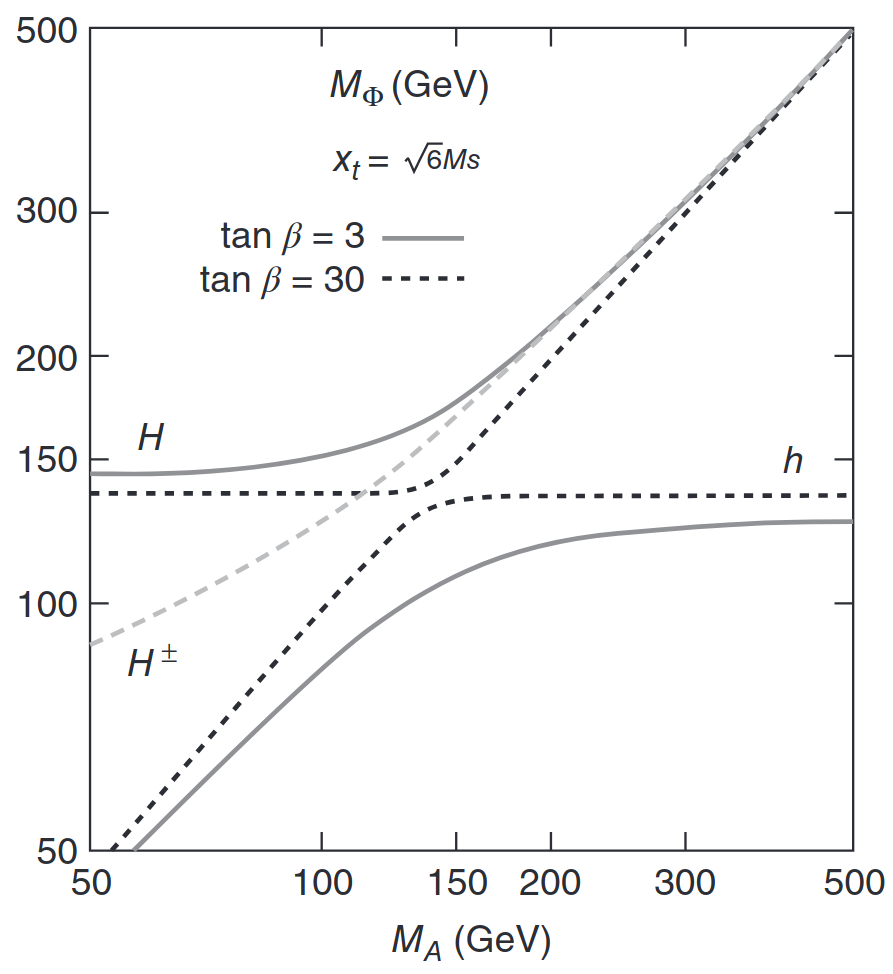
\includegraphics[width=8cm]{\PhDthesisdir/plots_and_images/from_Nagashima_BSM/fig_1-9.png}};

% masks
\fill [white] (1.5, 6) rectangle (3.3, 7);
\fill [white] (2.75, 7) rectangle (4.5, 8.2);
\fill [white] (1.1, 2.6) rectangle (1.7, 3);
\fill [white] (1.2, 4.6) rectangle (1.5, 5);
\fill [white] (7, 4.4) rectangle (7.3, 4.8);
\fill [white] (.5, 0) rectangle (8, 1);
\fill [white] (0, .9) rectangle (.75, 8.6);

% Notations
\draw (3.7, 8) node {\small $m_\Phi$ (\SI{}{\GeV})} ;
\draw (3.7, 7.25) node {\small $X_t = \sqrt{6} m_S$} ;
\draw (3.5, 6.6) node [left] {\small $\tan\beta = 3$} ;
\draw (3.5, 6.2) node [left] {\small $\tan\beta = 30$} ;
\draw (1.35, 4.85) node {\small $\Higgs$} ;
\draw (1.35, 2.85) node {\small $\Higgspm$} ;
\draw (7.1, 4.6) node {\small $\higgs$} ;

% X axis
\foreach \val in {50, 100, 150, 200, 300, 500}{
\draw ({0.8+(7.65-0.8)*(ln(\val/50))/(ln(500/50))}, .85) node {\small \val};
}
\draw (7.65, .25) node [left] {\normalsize $m_{\HiggsA}$ (\SI{}{\GeV})};
%
%% Y axis
\foreach \val in {50, 100, 150, 200, 300, 500}{
\draw (.8, {1.1+(8.45-1.1)*(ln(\val/50))/(ln(500/50))}) node [left] {\small \val};
}

\end{tikzpicture}
